\documentclass[12pt]{article}
\usepackage[utf8]{inputenc}
\usepackage{parskip}

\usepackage[bottom]{footmisc}
\usepackage{titlesec}

\usepackage{graphicx}
\usepackage{subcaption}
\usepackage{wrapfig}


\begin{document}

\section{Segmentation is my fault}
\subsection{Introducción y presentación del trabajo realizado}

La segmentación de imágenes de forma es un problema abierto en el área de
\emph{visión artificial} que dada la variedad de sus aplicaciones posee varios
intereses en conflicto al querer desarrollar un algoritmo definitivo para ésta.
Un algoritmo eficiente que requiera tiempo y memoria lineal puede ser útil para
procesamiento de video en tiempo real sacrificando la calida del resultado,
mientras que otro enfoque más costoso puede ser útil a la hora de ofrecer una
herramienta que facilite labores artísticos (separación automática de los
objetos en una escena, por ejemplo).

\begin{figure}[h]
	\centering
	\begin{subfigure}{0.4\linewidth}
		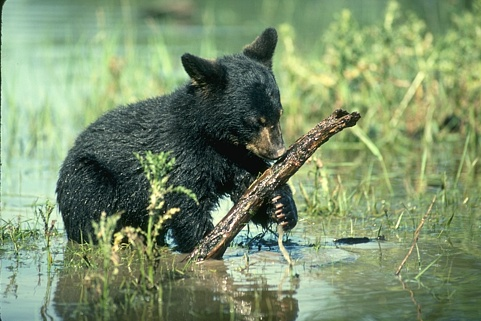
\includegraphics[width=\linewidth]{segmentation/entradas-posta/oso}
		\caption{Entrada}
	\end{subfigure}
	\begin{subfigure}{0.4\linewidth}
		\includegraphics[width=\linewidth]{segmentation/salidas/{0.8.oso.jpg.600.100}.png}
		\caption{Segmentación}
	\end{subfigure}
	\caption{$\sigma = 0.8,\ k = 600,\ g = 100$.}
\end{figure}

El algoritmo a implementar es el propuesto por \textbf{Pedro F.  Felzenszwalb}
y \textbf{Daniel P. Huttenlocher} en su trabajo \textsc{Efficient Graph-Based
Image Segmentation}. Éste algoritmo construye un grafo grilla con cada píxel en
su propio segmento y luego uno los segmentos golosamente dada una condición de
``similaridad suficente'' entre ellos. Para mejorar los resultados del
algoritmo se implementaron dos pasos de pre y post procesamiento.

El preprocesamiento consiste de un desenfoque gaussiano de dos pasadas. Éste se
implementó dentro del programa entregado luego de notar que desenfocar la
imagen y luego guardarla en el formato de entrada propuesto por la cátedra
resultaba en artefactos indeseables propios del bajo rango de valores de cada
pixel. El sigma de desenfoque puede ser modificando variando el segundo
parámetro pasado al ejecutable.

El postprocesamiento es una segunda pasada por las aristas del grafo forzando
la unión de todos los componentes suficientemente chicos. El significado de
``suficientemente chico'' se puede modificar variando el tercer parámetro
pasado al ejecutable. El parámetro es relativo a la resolución de la imagen a
procesar, un valor de $1$ eliminará todas las componentes que posean menos del
$100\%$ de los píxeles, uno de $10$ todas las que posean menos del $10\%$.
Llamaremos $g$ a este parámetro dado que cuanto mayor es su valor mayor es la
\emph{granularidad} de la segmentación resultante\footnote{Efectivamente el
parámetro pone un límite superior a la cantidad de segmentos que puede tener la
segmentación.}.

El algoritmo en sí posee un valor $k$ que representa la ``soltura'' a la hora
de comparar componentes para decidir si unirlas o no. Éste parámetro es el
primero que recibe el ejecutable entregado.

La elección de colores para las segmentaciones mostradas en este informe se
realizó aprovechándose de detalles implementativos. Esta elección nos permite
que los colores sean estables al variar tanto $k$ cómo $g$, lo cuál permitió
crear los videos adjuntos a este informe.

\subsection{Presentación informal e intuitiva del algoritmo}

El algoritmo implementado construye un \emph{grafo grilla} a partir de la
imagen proporcionada y luego recorre las aristas del mismo de menor a mayor
uniendo las compomentes de cada lado de la arista. La motivación es simple,
procesar los píxeles más similares al principio nos forzará a recorrer las
regiones de la imagen desde las de menos variabilidad hasta las que sean
básicamente ruido blanco.

Para tomar la decisión de si unir o no dos componentes se propone calcular la
\emph{diferencia interna} de una componente de la siguiente forma:

\[Int(C) = \max_{a \in AGM(C_V, C_E)} p(a)\]

Dónde $AGM(V, E)$ es el árbol generador mínimo del subgrafo de la componente
$C$, $C_V$ son los vértices de la componente V, $C_E$ son los ejes de la
componente $C$ y $p(e)$ es la función que determina el peso de una
arista\footnote{Dependiendo el espacio de color de la imagen y la forma en la
que se representen los mismos puede haber muchas funciones que tenga sentido
evaluar como $p$.}.

\begin{figure}[h]
	\centering
	\includegraphics[width=0.9\linewidth]{graficos/grilla}
	\caption{Grafo grilla con 8-vecindad.}
\end{figure}

Dado todo esto, dos componentes que limiten en un par de píxeles se unirán si
la diferencia en el límite está dentro de la tolerancia común de las mismas, es
decir si $\textit{diff} \geq Int(C_1) + \tau(C_1) \land \textit{diff} \geq
Int(C_2) + \tau(C_2)$, dónde $\tau(C)$ es la función que le da juego\footnote{\
En el sentido de que suma cierta holgura que permite unir componentes de que
otro parecerían demasiado distintas, cosa que es común con componentes
pequeñas} a la componente. La función propuesta para $\tau(C)$ es la siguiente:

\[\tau(C) = \frac{K}{|C_V|}\]

La que nos ofrece un valor cercano a $K$ para compontentes muy chicas y uno
cercano a $0$ para componentes muy grandes. Ésto fuerza a tener evidencias
claras de que dos componentes son en realidad la misma al ser estas muy grandes
pero nos permite un montón de juego en las primeras etapas.

\subsubsection{Entonces. ¿Cuál es el algoritmo aquí propuesto?}

Construiremos una primera aproximación burda (ubicando cada píxel en su propia
componente) y lo refinaremos preguntándonos si dado un par de componentes
unidas por un eje éstas no deberían en realidad unirse. A la hora de ejecutar
un algorimo así de goloso es importante el orden en el cuál se toman las
aristas a procesar. El obvio (y el utilizado por nosotros) es de menor a mayor
peso\footnote{En una implementación que requiera un tiempo de procesamiento
lineal se puede utilizar un \emph{Counting Sort} sabiendo cuál es la mayor
diferencia posible (256 en el caso de la entrada de la cátedra).}.

Entonces, sumando todos los procesos antes mencionados podemos construir una
suerte de vista aérea de nuestro algoritmo (que nos será útil para luego
ahondar en la implementación de cada parte).

\begin{enumerate}
	\item Cargar la entrada
	\item \textbf{Opcional:} Realizar un desenfoque para evitar
	      ciertos defectos.
	\item Construir el grafo grilla de la entrada, usando la diferencia
	      de intensidades entre píxeles vecinos como peso de cada arista.
	\item Ordenar las aristas construídas por peso.
	\item Construir la solución inicial, asignando a cada píxel (vértice
	      del grafo) en supropia componente.
	\item Por cada arista (de menor a mayor) determinar si los píxeles que
	      une deberían pertenecer a la misma componente. Si es así unirlos.
	\item \textbf{Opcional:} Por cada arista (de menor a mayor) si alguna
	      de las componentes que une es menor al $\frac{100}{g}\%$ de la
	      imagen entonces unir éstas.
	\item Imprimir la salida en el formato deseado, construir colores de
	      ser necesario, etc.
\end{enumerate}


\section{Llenalo con super}

\subsection{Presentación informal del problema}
Dado un vendedor que cuenta con vehiculo propio que necesita moverse entre ciudades personalmente para vender sus productos, quiere buscar la manera más económica de realizar la tarea.

Si la distancias entre ciudades estan representadas en kilometros y el precio de la nafta es por litro queremos minimizar el costo en nafta de llegar de cada ciudad a las demas teniendo en cuenta las siguientes propiedades: 

\begin{enumerate}
	\item Las rutas que comunican las ciudades son bidireccionales.
	\item El precio de la nafta varia de ciudad en ciudad.
	\item El auto posee un limite de litros de nafta que puede cargar (60 litros).
	\item Se estima que cada litro de nafta alcanza para exactamente un kilometro de distancia.
\end{enumerate}

El problema formalmente será representado como un grafo donde cada ciudad $c_i$ es un vertice con su respectivo precio por litro $p_i$ y donde cada distancia $d_{x,y}$ que comunica un par de ciudades ($c_x, c_y$) son las $m$ aristas del grafo.

Representado el $r_k$ como un camino posible entre dos ciudades en función del costo efectivo comprendido como la cantidad de litros $l_i$ que cargue de nafta por su respectivo precio $p_i$ queremos los caminos que cumplen que:

$\forall(c_x, c_y \in Ciudades)(r_{m}, r_k \in Caminos(c_x,c_y))\rightarrow(r_{m} < r_k)$

Es decir nos interesan todos los caminos minimos.

Una motivación razonable para resolver el problema sería entonces simplemente aplicar algoritmos conocidos de camino minimo, sin embargo esto no es posible con el grafo original.

Para empezar el precio al estar en función de los vertices, los costes no dependen solo de las distancias, sino de una multiplicación entre litros cargados por el precio.

Las rutas son bidireccionales, sin embargo dadas 2 ciudades $C_a$ y $C_b$ no se cumple que los costes $C_a \rightarrow C_b$ y $C_b \rightarrow C_a$ sean iguales.

Eso significa que necesitariamos una representación direccional si quisieramos hablar de costes efectivos. $Fig1, Fig2$ ilustran esta diferencia para 2 ciudades.

\begin{minipage}{0.45\textwidth}
	\centering
	\includegraphics[width=\linewidth]{{graficos/bidireccional}.pdf}
	\captionof{figure}{bidireccional}
\end{minipage}
\begin{minipage}{0.42\textwidth}
	\centering
	\includegraphics[width=\linewidth]{{graficos/direccional}.pdf}
	\captionof{figure}{direccional}
\end{minipage}


En particular $\forall(p_a \neq p_b) \rightarrow (p_a * d_{a,b} \neq p_b * d_{a,b}) $

Además los caminos minimos no necesariamente son simples, por ejemplo dadas 3 ciudades $C_a$, $C_b$ y $C_c$ y 2 rutas con distancia $d_{a,b}$ y $d_{a,c}$.


\begin{figure}
	\includegraphics[width=0.5\textwidth]{{graficos/caminoNoSimple}.pdf}
	\caption{Camino no simple}
\end{figure}

Tengo que si $p_a > p_b$ podría tener que evaluar si moverme allí para cargar nafta y volver es menos costoso, que ir directamente.

En fig3 se ilustra un grafo donde el costo de ir de $C_A$ a $C_C$ directamente es $p_a * d_{a,c} = 750$.

Mientras que el camino pasando por $C_b$ es:

$C_a$ a $C_b$ a $C_a$ a $C_C$ = 450.

Sin embargo esto motiva a analizar si existen transformaciones del grafo en la que aplicar algoritmos de camino minimo es posible.

\subsubsection{Pautas de diseño}

El objetivo de este trabajo es plantear transformaciones de grafos que nos permitan aplicar algoritmos de camino minimo. Buscaremos establecer una cota de las dimensiones de nuestro nuevo grafo en función de la densidad y tamaño del grafo original.

Someteremos nuestro grafo a diferentes experimentos buscando comparar entre diferentes algoritmos de camino minimo cual de ellos se ajusta mejor. No explicaremos algoritmos de camino minimo como Dijkstra, Bellman-ford o Floyd-Warshall, se entienden por conocidos.

Finalmente Dijkstra, bellman-ford son algoritmos $1$ a $N$ (nodos), cuando nos refiramos a ellos como algoritmos $N$ a $N$, nos referimos justamente a ejecutarlos $N$ veces (Abordaremos este tema en detalle en secciones posteriores).

\subsubsection{Transformación del grafo}

Lo que queremos es dado un grafo $V$, obtener todos sus costos efectivos minimos $R$ para cada $(C_i, C_j)$. Buscamos para resolver el problema 2 funciones. La primera una funciòn $f(V) = V'$ que convierta nuestro grafo en función del costo efectivo a un nuevo grafo en el cual si se puedan aplicar algoritmos de camino minimo. Luego buscamos una función $g(R') = R$ que sepa interpretar los resultados del nuevo grafo como solución del original y obtener los resultados de $V$ que nos interesan.

Dadas ambas funciones los pasos que aplicaremos sobre un grafo V para obtener los resultados R que nos interesan son los siguientes:

\begin{enumerate}
	\item $V' := f(V)$
	\item $R'$ := Algún algoritmo valido de camino minimo N a N.
	\item $R := g(R')$
\end{enumerate}

Ahora bien partamos de la primera incognita, como generar una funciòn $f(V)$.

Para lograr esta tarea, necesitamos eliminar la noción del precio ya que los algoritmos de camino minimo solo saben operar en funciòn del peso de las aristas. Además paso las aristas resultantes que debemos obtener serìa conveniente que esten en función del costo efectivo.

Sabemos además que la cantidad de litros de nafta que puede llevar nuestro vehiculo esta acotada por una constante llamemos $W$ de 60 litros. 

Debido a que W es acotado una estrategia razonable sería lograr que $f(V)$ dependa de esta constante, ya que la complejidad de un algoritmo de camino minimo $N$ a $N$ es $O(n^3)$, si incluimos el costo de la transformación sería $O(W * n^3)$ y si $W$ es constante no influiría en nuestra complejidad.

Empezemos por redefinir los vertices, en $V'$ no puedo tener estados, no puedo estar en una ciudad $C_i$ con $X$ de nafta, y un precio $p_i$ para agregar litros.

Lo primero que haremos será multiplicar cara vertice $C_i$ por W estados posibles\footnote{Si $(W = 60)$ los estados son $61$, puedo estar en $C_i$ con: (0..60) lirtros de nafta.} entonces si:

$V$ posee  N nodos. 

$V'$ posee N * 61 tal que si $C_i$ es nodo en V $\rightarrow$ $\exists$ $\sum_{k=0}^{W} C'_{i * k}$ nodos en $V'$

por notación llamaremos $C'_{i_0}$ a $C'_{i_{60}}$ a nuestros vertices en $V'$, ahora bien necesitamos redefinir nuestras aristas en función del costo efectivo.

Dado que nuestra transformación tiene $W$ estados que representan un mismo nodo necesitaremos aristas para movernos entre dichos estados, si razonamos que para ir $C'_{i_0}$ a $C'_{i_1}$ es exactamente agregar un litro de nafta es trivial asumir que en general tendremos que dado un estado $C'_{i_k}$ el costo para ir a $C'_{i_{k+1}}$ será exactamente $p_i$.

Es decir de momento nuestra transformaciòn tiene  $N * (W - 1$) aristas para movernos entre los estados $C'_{i_k}$

Lo siguiente que haremos serà redefinir como son las conexiones entre los nodos, por cada $d_{i,j} \in m$ de $V$


TODO: Terminar transformación, armar dem de correctitud y experimentación.


\end{document}
